\documentclass[12pt]{article}
\usepackage[margin=1in]{geometry}
\usepackage{fancyvrb}
\usepackage{multicol}
\usepackage{hyperref}
\usepackage{amsmath}
\usepackage{amsfonts}

\usepackage[listings]{tcolorbox}

\definecolor{codegreen}{rgb}{0,0.6,0}
\definecolor{codegray}{rgb}{0.5,0.5,0.5}
\definecolor{codepurple}{rgb}{0.58,0,0.82}
\definecolor{backcolour}{rgb}{0.95,0.95,0.92}

\lstdefinestyle{mystyle}{
    language=Python,
    backgroundcolor=\color{backcolour},   
    commentstyle=\color{codegreen},
    keywordstyle=\color{magenta},
    numberstyle=\tiny\color{codegray},
    stringstyle=\color{codepurple},
    basicstyle=\ttfamily\footnotesize,
    breakatwhitespace=false,         
    breaklines=true,                 
    captionpos=b,                    
    keepspaces=true,                 
    numbers=left,                    
    numbersep=5pt,                  
    showspaces=false,                
    showstringspaces=false,
    showtabs=false,                  
    tabsize=2,
    escapechar=|,
    frame=single
}

\lstset{style=mystyle}

\newcommand{\showfig}[2]{
\noindent\includegraphics[width=\textwidth]{#1}
\centerline{#1}
}

\begin{document}
\sloppy
\centerline{\Large CSCI 111, Lab 11}
\centerline{\large 3d height field visualizer}


\begin{description}
\item[Due date:] Midnight, Tuesday, December 6, on Canvas.
No late work accepted.  

\item[File names:]  Names of files, functions, and variables, 
when specified,
must be EXACTLY as specified.  This includes simple mistakes such
as capitalization.

\item[Individual work:]  All work must be your own.  Do not share
code with anyone other than the instructor and teaching assistants.
This includes looking over shoulders at screens with the code open.
You may discuss ideas, algorithms, approaches, {\em etc.} with
other students but NEVER actual code.

\item[3d vector type:]  You will need your solution to Lab 10,
the vector module, for this assignment.  Add the following method
to the class.  It returns the cross product of two vectors,
a vector perpendicular to both.

\begin{lstlisting}
    def cross(self, other):
        a1, a2, a3 = self.x, self.y, self.z
        b1, b2, b3 = other.x, other.y, other.z
        s1 = a2*b3 - a3*b2
        s2 = a3*b1 - a1*b3
        s3 = a1*b2 - a2*b1
        return V(s1,s2,s3)
\end{lstlisting}
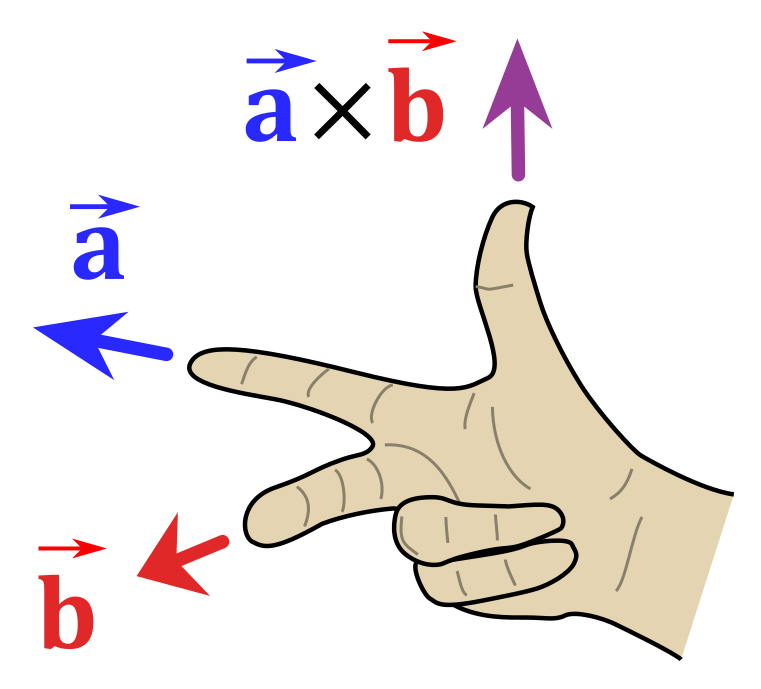
\includegraphics[scale=0.2]{crossproduct}

If you didn't finish this project you can use my implementation,
available on the lab website.

\item[The program]  In the folder \lstinline{poly3d} on the
lab website you can find a skeleton of this program.  The main
program, \lstinline{poly3d.py} is complete, as well as the 
\lstinline{vector.py}, \lstinline{functions.py}, \lstinline{gradient.py}
 and \lstinline{polygon.py}
modules.

You will only have to complete the \lstinline{parametricsurface.py} module.

\item[Step 1, heightfield:]  
Start with implementing 
\begin{lstlisting}
    def makeHeightfield(self):
        """calculate nxn 3d points in xrange x yrange
           store V(x,y,z) in self.heightfield[i,j]"""
\end{lstlisting}

This should create an empty dictionary.  Loop over
i and j in range(n), and lerp i and j into the xrange 
and yrange, getting x and y in parameter space.
Applying the function to x and y gives a point p in world
space.  Store p in self.heightfield[i,j]

Test this with a simple function, for example x+y,
in the range 1..10 with n=10.  Print out the heightfield
so you can see it's working.

\item[Step 2, project points:] 
Next implement
\begin{lstlisting}
    def projectPoints(self, eye):
        """project 3d points in heightfield to
              2d points (x,y) in plane of camera
              store in self.points[i,j]
           also calculate for these points
              self.minx, maxx, miny, maxy
           also calculate color based on gradient and height
              store in self.color[i,j]
           also calculate eye distance
              store in self.distance[i,j]
        """
\end{lstlisting}
Project the 3d points in \lstinline{sefl.heightfield} using the eye
point.  

Create a frame of vectors around the eye, forward, up, and right:
\begin{lstlisting}
    fwd = -eye
    up = V(0,0,1)
    rt = fwd.cross(up)
    fwd.gram_schmidt(up, rt)
\end{lstlisting}
Then use the Gram-Schmidt procedure to make them
The method to make an orthonormal frame around 
the eye is part of the \lstinline{Poly3d} object.

If pt is our 3d point from the heightfield,
the x coordinate of our pt will be the projection
of a vector to the point onto the right-pointing vector
and the y coordinate will be the projection onto the up-pointing
vector:
\begin{lstlisting}
x = (pt - eye) * rt
y = (pt - eye) * up
\end{lstlisting}
For each [i,j]
store the x,y tuple in \lstinline{self.points[i,j]}.

Also calculate the distance from the point to the eye.
This is just the length of the vector from the point to the eye,
\lstinline{(pt - eye).length()}.
Store these in \lstinline{self.distance[i,j]}

Also, since we're calculating every x,y value for every point,
we can also remember the minima and maxima for both
x and y.  Save these, as well, in \lstinline{self.xmin} etc.

Test this on some simple heightframes with some simple
eyes.  For example, what would you expect if the eye 
is V(1,0,0)?  What about V(0,1,0)?

\item[Step 3, scale points:]  Now implement the function
\begin{lstlisting}
    def scale(self, size):
        '''lerp the polygons from xrange x yrange into 0..w x h..0
           can shrink the screen range 10% if you like
        '''
\end{lstlisting}
 We start with a set of 2d points
stored in \lstinline{self.points}.  These are the points in the camera
frame, and their limits are stored in \lstinline{self.xmin}, \lstinline{self.xmax},
{\em etc.}  We want to lerp these points into the ranges (0,width-1)
and (height-1,0), where \lstinline{width,height = size}

Loop over all i and j and for all points in \lstinline{self.points[i,j]},
lerp the x value from \lstinline{(self.xmin, self.xmax)}
into the range \lstinline{(0, width-1)}, and the y value
into the range \lstinline{(height-1, 0)}.  You can store
the result right back in \lstinline{self.points[i,j]}.

We now have a set of points in screen coordinates, and we're ready
to plot them.

\item[Step 4, make polygons:] Now finish the function
\begin{lstlisting}
    def makePolygons(self, eye, size):
        """
           then build polygons from self.points, self.color, self.distance
           using [i,j], [i+1,j], [i+1,j+1], [i,j+1] indices
           then sort the polygons based on distance (farthest first)
        """
        self.projectPoints(eye)
        self.scale(size)
\end{lstlisting}
This function will be called from another object to create
the polygons from a heightfield.  It first calls
\lstinline{projectPoints} and then \lstinline{scale}
to get points in screen space, ready to be drawn.

Now make polygons out of the projected points.
For each point with i,j in range(n-1), use the points
at [i,j], [i+1,j], [i+1,j+1], [i,j+1] to make a polygon.
Use the average of these four distances as the
distance to the polygon.  You can use blue, \lstinline{'#0000ff'}
for the color.

Sort your polygons by distance, farthest first.

The best way to test now is to rerun the \lstinline{poly3d}
module, which will plot all your polygons.  Not good?  Debug!

\item[Step 5, add color:] Go back to  \lstinline{projectPoints}.
 Use the gradient object to find the color
of the point, based on the z value in 3d.  Store these in
\lstinline{self.color[i,j]}  

Now go back to \lstinline{makePolygons}  and 
add this color to the polygon, instead of blue.
You can average the four colors from the four corners,
or just use one of the four colors.

Replot. Colorful?

\item[Step 6, shading:] Go back to \lstinline{projectPoints}, where you
found the color using the gradient and the z value of the 3d point.

Get three points from the heightfield, \lstinline{p0} at [i,j], \lstinline{p1} at [i+1,j],
and \lstinline{p2} at [i, j+1].

Warning!  You can't use these when i or j are equal to n-1.  It will be
good enough if you just replace i with i-1 or j with j-1 in this case.

Now find two {\bf tangent vectors} to the surface, \lstinline{v1 = p1-p0}
and \lstinline{v2 = p2-p0}.
Find the {\bf normal} to the surface at [i,j] using the cross
product of the vectors, \lstinline{normal = v1.cross(v2)}. 
Normalize the length of this vector.

Now take the dot product of the normal with
a normalized vector pointing toward the light.
You can put the light anywhere you want.  Mine is in
this direction: \lstinline{V(2,-1,4)} .  Remember to normalize
the light vector!

The dot product of the normal and the light gives you the shade value,
but it if's less than 0.25 use 0.25 instead of the value.  In other words,
\begin{lstlisting}
  shade = max(0.25, normal * light)
\end{lstlisting}

Use this shade value to darken the color.  It's an optional parameter
to the gradient object.

\item[Optional, moving on:]
Colorize with a different gradient!

Find some interesting parametric surfaces!

\end{description}



\end{document}
